Vzhledem k nejednoznačné definici pojmu \textit{\enquote{extrémní prostředí}} je
potřeba stanovit vhodnou interpretaci v souvislosti s problematikou této práce.
Mezi rané definice přispěli Harrison a Connors~\cite{harrison1984}, kteří
publikovali, že extrémní prostředí se vyznačuje nebezpečnými a nepřívětivými
klimatickými, životními nebo pracovními podmínkami a možnou sociální izolací.
Bell~et~al.~\cite{bell2016} definovali extrémní situace jako okolnosti, za
kterých má nedostatečný výkon, ať už mentální nebo fyzický, vážné následky
(např. časová tíseň, nebo nebezpečí). Všechny tyto koncepty se týkají náročných
fyzických nebo mentálních výkonnostních situací, na které se pojí další již
formulované pojmy jako mimořádné
situace~\cite{stachowski2009benefits,yu2008misery}, psychický a fyzický
nátlak~\cite{gardner2012performance} nebo stres~\cite{Staal2013StressCA}. Další
formulace byly již uvedeny
v~\cite{hannah2009framework,hallgren2018matter,golden2018teams}. V této práci je
na definici extrémního prostředí nahlíženo jako na izolované atypické prostředí,
v němž jsou kladeny značné nároky na plněné úkoly, které s sebou nesou vysokou
míru rizika a katastrofické důsledky při chybném či nedostatečném výkonu.

Současné studie se v rámci tématiky extrémního prostředí často zabývají vlivem
izolovaného a stísněného prostředí (\gls{ICE}, isolated, confined, and extreme)
na člověka~\cite{Pagel2016,golden2018teams} nebo vlivem různorodých
enviromentálních podmínek~\cite{Taylor2016,Winnard2019,Zhang2019}. Do výzkumu v
této oblasti se začalo aktivně přispívat kolem první poloviny 20. století, což
bylo podmíněno vědecko-technologickým pokrokem. Mezi hlavní iniciační milníky
patřil vojenský zájem o dlouhodobé ponory jaderných ponorek, na který navázal
podvodní výzkum~\cite{Maynard2018,Driskell2018}, vznik vesmírných programů
(vesmírný závod) a polární výzkum~\cite{wickman2008,stuster2007bold}. Pro
potřeby této práce je dále detailněji rozebíráno extrémní prostředí z hlediska
vesmírné explorace, konkrétně dlouhodobých vesmírných letů a analogových
vesmírných misí.

\subsection{Vesmírné explorace}
\label{subsection:vesmirne_explorace}
Za hlavní hnací historický faktor, který posouval vědecko-technickou sféru v
rámci výzkumu vesmíru rychle kupředu lze považovat tzv. vesmírný závod, jenž
začal vypuštěním družice Sputnik 1 Sovětským svazem v roce 1957. Rok poté byl
založen Americký Národní úřad pro letectví a vesmír (\gls{NASA}), což vedlo k
prvním vesmírným misím, kterých se později účastnily i posádky. Byl tak vytvořen
nový prostor a vzbuzen výzkumný zájem v oblasti analogových vesmírných misí,
jelikož otázky ohledně průzkumu vesmíru odhalily spoustu vědomostních nedostatků
potřebných pro úspěšný pobyt v kosmu~\cite{Driskell2018}. Nejedná se však ani
tolik o technické překážky, ale o nedostatky znalostí zejména v oboru neurověd a
experimentálního nastavení.

\begin{figure}[!htb]
    \begin{center}
        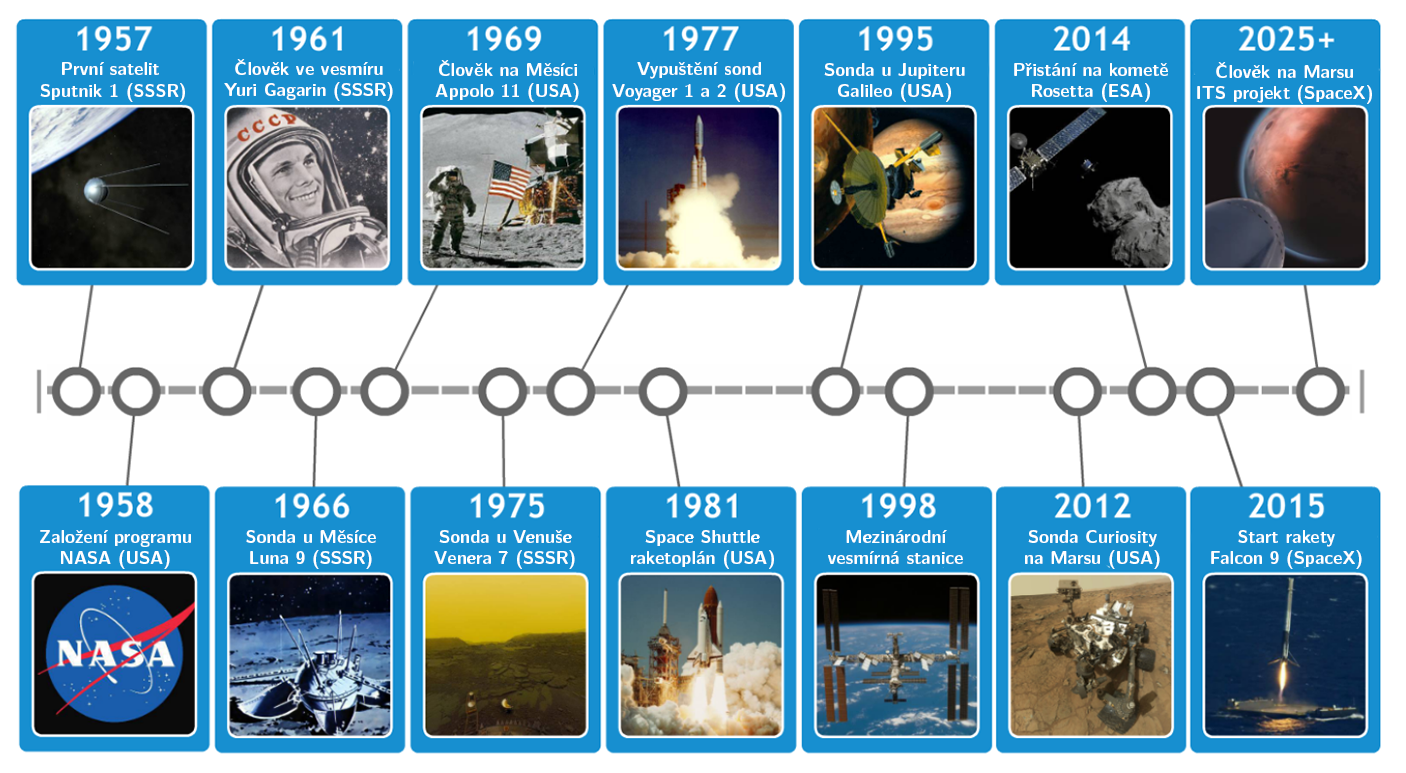
\includegraphics[width=1\linewidth]{figures/space_exploration}
        \caption{Časová osa výzkumu vesmíru od Sputniku po Mars (Přeloženo a
            převzato z~\cite{bartu})}
        \label{fig:space_exploration}
    \end{center}
\end{figure}

Vzhledem k tomu, že budoucnost výzkumu vesmírné explorace sahá za hranice oběžné
dráhy Země~\cite{salotti2014roadmap,viscio2014methodology}, je třeba brát v
úvahu obtíže budoucích misí, které se budou primárně týkat člověka. Dlouhodobé
kosmické lety a mise jsou předmětem mnoha zásadních okolností, jež kladou vysoký
a rizikový neuropsychofyziologický nátlak~\cite{Mogilever2018}. Extrémní
prostředí, komunikační latence a problémy (např. dlouhodobý výpadek komunikace)
nebo fyziologické změny vlivem vesmírných
aspektů~\cite{Buguet2007,Williams2009,Roy2021} mohou během dlouhodobých misí
překračovat lidské psychické i fyzické hranice a vést ke katastrofickým
následkům~\cite{Strangman2014,Mogilever2018}. Toto riziko se uplatňuje i
přestože se v těchto případech skládají posádky z vybraných trénovaných jedinců
(astronautů). Stresory, vnitřní nebo vnější stimuly vznikající při vystavení
lidského organizmu mimořádným podmínkám (extrémnímu prostředí) při dlouhodobých
vesmírných letech, již popsal Morphew~\cite{morphew2001psychological}. Zdravotní
a výkonnostní rizika lze řešit právě výběrem a výcvikem posádky nebo například
návrhem mise a vybavení. Naskytuje se ale také možnost tato rizika predikovat s
využitím diagnostických neinvazivních metod, mezi které patří funkční magnetická
rezonance~(\gls{fMRI}) nebo elektrokardiografie~(\gls{EKG}), spolu s širokými
znalostmi lidského nervového systému. Je tedy třeba realizovat experimenty,
které pomohou lépe chápat, ne-li přímo definovat NPF vztahy při vlivu extrémního
prostředí. Takové experimenty však nemohou probíhat za normálních laboratorních
podmínek, jelikož se nejedná o prostředí, které by odráželo skutečné provozní
podmínky a účinně napodobilo kosmickou misi~\cite{Mogilever2018,Pagel2016}.

Ke studiu neuropsychofyziologických adaptací člověka vystavenému mikrogravitaci
se využívají data zaznamenaná před a po vesmírném letu, kde se také sledují
změny jako distribuce tělesných tekutin, hustota kostí nebo úbytek svalové
hmoty~\cite{Stein2012WeightMA}. Kromě mikrogravitace lze mnoho vědeckých otázek
týkajících se kognitivních neurověd zodpovědět i na Zemi díky vesmírným
analogovým misím, které simulují komplexní interakce vznikající během vesmírných
misí~\cite{Pagel2016,Mogilever2018}.

\subsection{Analogové mise}
\label{subsection:analogove_mise}
Jak již bylo zmíněno, laboratorní experimenty plně nereprezentují reálné
podmínky dlouhodobých kosmických misí, avšak různá analogová prostředí
(analogové mise) přinášejí právě tu možnost sledovat a zkoumat NPF člověka v
jedinečných situacích~\cite{Mogilever2018}. Situace, které napodobují reálné
okolnosti budoucích vesmírných misí -- přistání kosmické lodi, extravehikulární
aktivity (\gls{EVA}), lékařské zákroky aj. -- vystavují jedince pozorovatelným
změnám například v cirkadiánním\footnote{Cirkadiánní rytmus je biologický rytmus
s cyklem trvajícím přibližně jeden den.} rytmu, hladinách stresových hormonů,
imunitních funkcích nebo neurokognitivním změnám~\cite{Pagel2016,Taylor2016}.
Faktory prostředí a jejich vliv na \gls{NPF} jsou detailněji popsány v
následující kapitole.

\begin{figure}[!htb]
    \begin{center}
        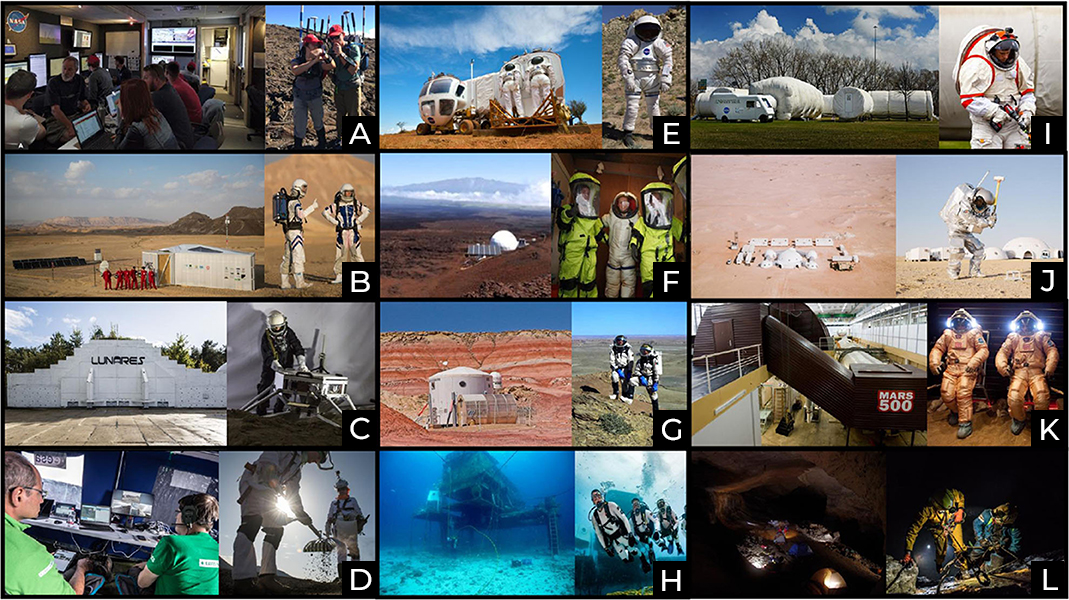
\includegraphics[width=1\linewidth]{figures/analog_missions}
        \caption{Příklady analogových misí. \textbf{(A)} NASA BASALT (USA),
            \textbf{(B)} D-MARS (Izrael), \textbf{(C)} LUNARES (Polsko),
            \textbf{(D)} ESA/PANGEA (Španělsko), \textbf{(E)} NASA/D-RATS (USA),
            \textbf{(F)} HI-SEAS (USA), \textbf{(G)} Mars Desert Research Station
            (USA), \textbf{(H)} NASA/NEEMO (USA), \textbf{(I)} NDU Habitat (USA),
            \textbf{(J)} OeWF/AMADEE-program (Rakousko, Omán), \textbf{(K)} Mars-500
            (Rusko), \textbf{(L)} ESA/CAVES (Španělsko/Itálie). (Upraveno a převzato
            z~\cite{groemer2020})}
        \label{fig:analog_missions}
    \end{center}
\end{figure}

Přehled několika analogových misí, na jejichž vzniku a vývoji se převážně
podílejí: Evropská kosmická agentura (\gls{ESA}), Státní korporace pro kosmické
aktivity (ROSCOMOS), Kanadská kosmická agentura (\gls{CSA}) a \gls{NASA}, lze
vidět na obrázku~\ref{fig:analog_missions}. Každá analogová mise vnikla primárně
pro simulaci a studium určitých vlivů vesmírných podmínek nebo k testování
specifického vybavení. Antarktické mise slouží k testování astrobiologických
hypotéz~\cite{Mogilever2018} a studiu dopadů izolace na člověka během extrémních
podmínek, které jsou dané drsným polárním podnebím a rozsáhlou
tundrou~\cite{Barkaszi2016,lugg1999}. Významnou misí je projekt Mars-500, kde
byla šestičlenná posádka uzavřena 520 dní v napodobenině kosmické lodi pro účely
simulace vesmírného letu na Mars. Během této mise došlo k řadě experimentů,
které se například zabývaly vlivem fyzického cvičení na aktivitu prefrontální
kortexu a kognitivní výkonnost~\cite{schneider2013} nebo změnami nálady a
plazmatických hladin hormonů~\cite{wang2014}. Na základě problematiky této práce
jsou nadále popsány vybrané podvodní analogové mise.

\subsubsection*{Projekt NEEMO}
Operace \gls{NASA} v extrémním prostředí neboli \gls{NEEMO} (NASA Extreme
Environment Mission Operations) jsou analogové vesmírné mise, které probíhají v
Mezinárodní Univerzitní Podmořské Výzkumné Laboratoři na Floridě (Florida
International University's Aquarius Undersea Research Laboratory, \gls{FIU}
\gls{AURL}). Podvodní laboratoř s rozlohou zhruba \SI{43}{\metre\squared},
umístěná \SI{19}{\metre} pod mořskou hladinou přesně nenapodobuje vesmírné
podmínky, ale primárně stresové faktory spojené s bezpečností, komunikací a
technologickou logistikou při dlouhodobých kosmických letech a průzkumu. Zároveň
zde probíhají testy vybavení a trénování výstupu do vesmíru mimo kosmickou
loď~\cite{trembanis2012neemo,koutnik2021neemo}. Poslední mise v podvodní
laboratoři, \gls{NEEMO} 23, proběhla v červnu 2019 a byla primárně zaměřena na
průzkumné výstupy do vesmíru.

\begin{figure}[!htb]
    \centering
    \begin{minipage}[b]{.48\linewidth}
        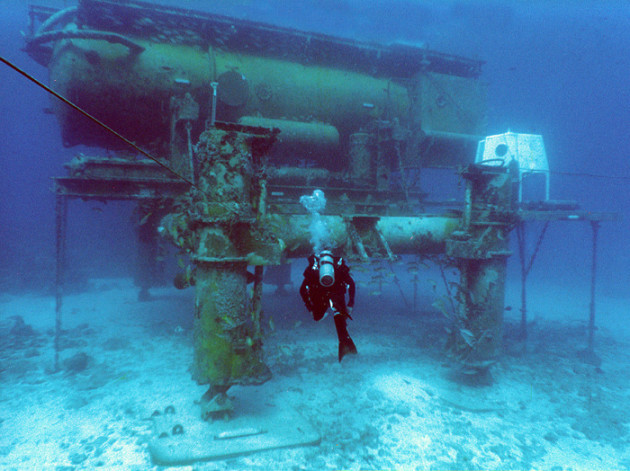
\includegraphics[width=\linewidth]{figures/neemo_habitat}
        \caption{Podvodní habitat AURL~\cite{NASAneemo}}
    \end{minipage}
    \hfill
    \begin{minipage}[b]{.48\linewidth}
        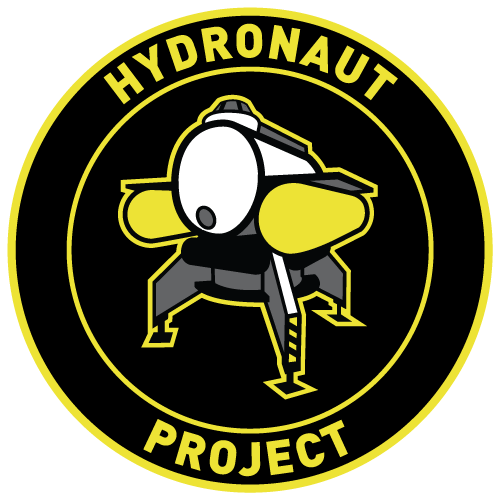
\includegraphics[width=\linewidth]{figures/hydronaut}
        \caption{Hydronaut H03 DeepLab~\cite{ESAhydronaut}}
    \end{minipage}
\end{figure}

\subsubsection*{Projekt Hydronaut}
Skromnější verze mobilního podvodního habitatu vznikla i v České republice za
účelem výcviku astronautů Evropské kosmické agentury. Projekt byl představen
roku 2010 a jeho primárním cílem bylo umožnit menším posádkám dlouhodobý pobyt
v hyperbarickém \gls{ICE} prostředí a simulaci vesmírných scénářů pro potřeby
výzkumu a vývoje. Podvodní stanice Hydronaut je plně mobilní a lze měnit její
umístění a hloubku zanoření. Současná stanice (H03 DeepLab) je vybavena několika
systémy pro sledování stavu habitatu a posádky. Jedním ze systémů je platforma
Common Tongue, který umožňuje nejen komunikaci s posádkou ale také sledování
fyziologických funkcí. V roce 2020 proběhla desetidenní mise (Mission One),
která včetně účelů kosmického \gls{ICE} výzkumu sloužila jako zátěžový test
habitatu~\cite{hydronaut2014}.


\subsection{Faktory prostředí a změny CNS}
\label{subsection:faktory_prostredi_zmeny_cns}
Vzhledem k tomu, že vesmír je jedinečné prostředí, je studium změn
neurofyziologického stavu člověka souvisejících s kosmickými misemi obtížné.
Předchozí studie ukázaly, že po letu do vesmíru dochází ke změnám ve vnímání,
pohybu, koordinaci a kognici~\cite{Moore2019}. Mikrogravitace je jedním z
hlavních faktorů, které ovlivňují mozek včetně kosmického záření (radiace),
izolace nebo hyperkapnie~\cite{Roy2021}. Důsledky působení mikrogravitace na
mozek popsal Torre v~\cite{Torre2014}. Souhrn faktorů lze vidět na
Obrázku~\ref{fig:factors_neuro} a jejich počet nasvědčuje, že pozorované
\gls{NPF} změny u astronautů mohou být důsledkem kombinace více stresorů na
jednotlivé oblasti mozku~\cite{Roy2021}.

Nedávné MRI studie poukázaly na změny polohy mozku, objemu tkáně, objemu
mozkových komor, distribuce a dynamiky mozkomíšního moku, mikrostruktury tkáně a
funkční konektivity po letu do
vesmíru~\cite{Ombergen2019,Pechenkova2019,Roberts2017,Demertzi2015,Kramer2020}.
Přehled \gls{MRI} studií provedených na amerických astronautech a ruských
kosmonautech před a po kosmickém letu se zjištěnými poznatky byl vypracován
v~\cite{Roy2021}. Mezi tyto studie jako jeden z prvních přispěl Demertzi et
al.~\cite{Demertzi2015} s objevem snížené konektivity v pravé
insule\footnote{Insula neboli insulární kortex je složitá struktura s rozsáhlou
sítí korových a podkorových oblastí mozku, které slouží smyslovým, emočním a
kognitivním funkcím.}, který se podílí na vestibulárním zpracování a kognitivní
kontrole.

\begin{figure}[!htb]
    \begin{center}
        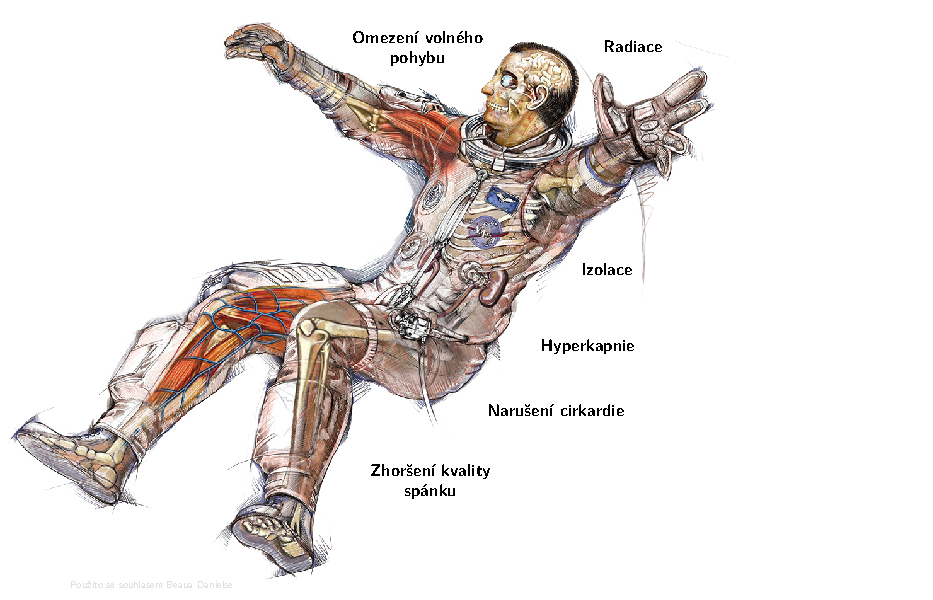
\includegraphics[width=1\linewidth]{figures/space_stressors}
        \caption{Souhrn stresových faktorů vesmírného \gls{ICE} prostředí, které
            mohou ovlivnit mozek během kosmického letu. Radiace v tomto případě
            odkazuje na radiaci v otevřeném kosmickém prostoru, nikoli na nízké
            oběžné dráze (\gls{LEO}). (Upraveno a převzato
            z~\cite{Roy2021,Hodkinson2017} se souhlasem Beaua Danielse)}
        \label{fig:factors_neuro}
    \end{center}
\end{figure}

Neurozobrazovací studie na zvířecích modelech a lidech vystavených analogovým
vesmírným letům prokázaly změny mozku související s reálným kosmickým
letem~\cite{Kramer2020,Correia1998}. Analogové vesmírné mise nacházejí tedy
uplatnění při zkoumání vlivů stresorů spojených s vesmírným prostředím na
centrální nervovou soustavu (CNS). Při srovnání změn CNS souvisejících s
kosmickou misí se změnami pozorovanými u pozemských analogů se naskytuje
příležitost do budoucna navrhnout strategie a opatření, které by předcházely
nežádaným NPF účinkům. Během analogových misí se podařilo reprodukovat například
zjištění spojené se změnami mozkové konektivity, objemu šedé hmoty, dynamiky
mozkomíšního moku a objemu mozkových komor~\cite{Roy2021}. Metoda, která věrně
napodobuje podmínky kosmických letů vystavováním subjektů posunu tělních
tekutin, odlehčení axiálního tlaku nebo hypokinezi, se nazývá Head-Down Bed Rest
(\gls{HDBR}). Subjekt je během metody na lůžku hlavou dolu, pod určitým
náklonem. HDBR zároveň vyvolává podobné změny v mozkové konektivitě, včetně
změny konektivity motorických, somatosenzorických a vestibulárních oblastí mozku
jako při vesmírných letech~\cite{Koppelmans2016, Koppelmans2017}.

Mozek je kromě fyziologických stresorů ovlivněn také dlouhodobým pobytem v
\gls{ICE} prostředí. Po 520denní misi Mars-500 ukázaly snímky participantů
pozměněnou mikrostrukturu šedé hmoty v pravém temporoparietálním
spojení\footnote{Temporoparietální spojení je část mozku, kde se setkávají
spánkový a temenní lalok.} (\gls{TPJ}), což je přisuzováno vlivu izolovaného
prostředí~\cite{Brem2020}. Během dlouhodobých vesmírných misí mohou mít změny
TPJ za následek zhoršení neuropsychofyziologické adaptace člověka na nové ICE
prostředí. Další nežádoucí změny byly prokázány v rámci studií antarktických
expedic, které demonstrovaly snížení objemu šedé hmoty v orbitofrontální kůře,
prefrontální kůře a hipokampu. Vzhledem k povaze antarktického prostředí a
expedic lze usuzovat, že jsou tyto změny podmíněné také vlivem
\gls{ICE}~\cite{Stahn2019}. Možné snížení neurogeneze hipokampu vlivem
extrémního prostředí může mít vliv na paměť a sociální interakci členů
posádky~\cite{Roy2021}. Délka kosmické mise či letu také hraje rozdíl, jelikož
větší míra změn struktury mozku byla pozorována u dlouhodobých vesmírných
misí~\cite{Roberts2017}.